% ****** Start of file apssamp.tex ******
%
%   This file is part of the APS files in the REVTeX 4.1 distribution.
%   Version 4.1r of REVTeX, August 2010
%
%   Copyright (c) 2009, 2010 The American Physical Society.
%
%   See the REVTeX 4 README file for restrictions and more information.
%
% TeX'ing this file requires that you have AMS-LaTeX 2.0 installed
% as well as the rest of the prerequisites for REVTeX 4.1
%
% See the REVTeX 4 README file
% It also requires running BibTeX. The commands are as follows:
%
%  1)  latex apssamp.tex
%  2)  bibtex apssamp
%  3)  latex apssamp.tex
%  4)  latex apssamp.tex
%
\documentclass[%
%reprint,
%superscriptaddress,
%groupedaddress,
%unsortedaddress,
%runinaddress,
%frontmatterverbose, 
%preprint,
%showpacs,preprintnumbers,
 nofootinbib,
%nobibnotes,
%bibnotes,
 amsmath,amssymb,
 aps,
 pra,
%prb,
%rmp,
%prstab,
%prstper,
%floatfix,
]{revtex4-1}
\usepackage{graphicx}% Include figure files
\usepackage{dcolumn}% Align table columns on decimal point
\usepackage{bm}% bold math
%\usepackage{chemist}% Chemical
\usepackage{chemmacros} % Chemical
\usepackage{hyperref}% add hypertext capabilities
%\usepackage[mathlines]{lineno}% Enable numbering of text and display math
%\linenumbers\relax % Commence numbering lines
\usepackage{natbib}
\usepackage{acro}
\usepackage{nomencl}
\usepackage{tikz}
\usetikzlibrary{shapes,arrows}
%\bibliographystyle{plainnat}
%\usepackage[showframe,%Uncomment any one of the following lines to test 
%%scale=0.7, marginratio={1:1, 2:3}, ignoreall,% default settings
%%text={7in,10in},centering,
%%margin=1.5in,
%%total={6.5in,8.75in}, top=1.2in, left=0.9in, includefoot,
%%height=10in,a5paper,hmargin={3cm,0.8in},
%]{geometry}

% PLAIN FILE TO HAVE REFERENCES FOR COMBUSTION AND FLAME
% STYLE
\def\rtn{\par \noindent}
\def\pskip{\rtn}

%%%%% A %%%%%%%
\def\aa{ Acta Astronautica}
\def\ab{ Acta Biomaterialia}
\def\abc{ Anal. Bioanal. Chem.}
\def\aam{ Adv. Appl. Mech.}
\def\aas{ Atomization and Sprays}
\def\abe{ Ann. of Biomed. Eng.}
\def\ag{ Adv. Geophys.}
\def\ats{ Ann. of Thora. Surg.}
\def\aiaaj{ Am. Inst. Aeronaut. Astronaut. J.}
\def\aiaap{ AIAA Paper}
\def\aj{ AIAA J.}
\def\ajou{ Aeronaut. J.}
\def\aicej{ AChE. J.}
\def\ajp{ Am. J. Phys.} 
\def\ana{ Anesth. Analg.}
\def\am{ App. Math.}
\def\amic{ App. Microbio.}
\def\an{ Acta Num.}
\def\anchem{ Anal. Chem.}
\def\anm{App.Num. Math.}
\def\ao{Artif. Organs}
\def\ap{ Adv. Phys.}
\def\apl{ App. Phys. Lett.}
\def\arbbs{ Ann. Rev. Biophys. Biomol. Struct.}
\def\arbe{ Ann. Rev. Biomed. Eng.}
\def\arfm{ Ann. Rev. Fluid Mech.}
\def\arp{ Ann. Rev. of Phys.}
\def\asas{ Astron. and Astrophys.}
\def\asaio{ Am. Soc. Artif. Intern. Org. }
\def\autcf{Reprinted by permission of Elsevier Science from}
\def\autcff{\copyright ~the Combustion Institute}
\def\autjfm{Reprinted with permission by Cambridge University Press}
\def\at{Atom. Sprays}
\def\atvb{ Arterioscl. Throm. Vas.}
\def\ajphcp{ Am. J. Physiol. Heart Circ. Physiol.}

%%%%% B %%%%%%%
\def\bioc{ Biochemistry-US}
\def\biom{ Biomat.}
\def\bb{ Biotechnol. Bioeng.}
\def\bba{ Biochim. Biophys. Acta}
\def\bbpc{ Ber. Bunsenges. Phys. Chem.}
\def\bioe{ Bioelectrochem.}
\def\bioee{ Bioelectro. Bioenerg.}
\def\biomat{ Biomaterials}
\def\biom{ Biomed. Mater.}
\def\biomf{ Biomicrofluid.}
\def\biomic{ Biomed. Microdev.}
\def\biop{ Biophys. J.}
\def\bior{ Biorheo.}
\def\bios{ Biosens. Bioelec.}
\def\blood{ Blood}
\def\blre{ Bl. Rev.}
\def\bmb{ Bull. Math. Biol.}
\def\bmm{ Biomech. Model. Mechanobiol.}

%%%%% C %%%%%%%
\def\canm{ Comm. Appl. Num. Meth.}
\def\care{ Cardiov. Res.}
\def\ccp{ Commun. Comput. Phys.}
\def\cea{ Cell Anal.}
\def\cepp{ Clin. Exp. Pharm. Phys.} 
\def\ces{ Chem. Eng. Sci.}
\def\cf{ Combust. Flame}
\def\cfl{ Comput. Fluids}
\def\cg{ Comput. Graph.}
\def\ch{ Chaos}
\def\cip{ Comput. Phys.}
\def\cir{ Cardiov. Interv. Radiol.}
\def\cire{ Circ. Res.}
\def\clch{ Clin. Chem.}
\def\clhem{ Clin. Hemorheo.}
\def\clm{ Clin. Lab. Med.}
\def\cm{ Comput. Mech.}
\def\cma{ Comput. Math. Appl.}
\def\cmame{ Comput. Meth. Appl. Mech. Eng.}
\def\cmb{ Cell. Mol. Bioeng.}
\def\cmmm{ Comput. Math. Meth. Med.}
\def\cmbbe{ Comput. Meth. Biomech. Biomed. Eng.}
\def\cocis{ Curr. Op. Coll. \& Interf. Sc.}
\def\cosuA{ Coll. Surf. A: Physicochem. Eng. Asp.}
\def\ca{ CA Cancer J. Clin.}
\def\cpa{ Cytom. Part A}
\def\cpam{ Commun. Pure Appl. Math.}
\def\cpc{ Computer Phys. Communications}
\def\cps{ Colloid Polym. Sci.}
\def\cras{ C. R. Acad. Sci.}
\def\crm{ Comp. Rend. M\'ec.}
\def\crp{ Comp. Rend. Phys.}
\def\cs{ Comput. Struct.}
\def\cst{ Combust. Sci. Tech.}
\def\ctm{ Combust. Theory and Modelling}
\def\cve{ Cardiov. Eng.}
\def\cvet{ Cardiov. Eng. Tech.}
\def\cvs{ Comput. Visual. Sci.}
\def\spctr{ Proc. of the Summer Program, Stanford NASA C.T.R}
\def\ctrarb{ Ann. Res. Briefs}
\def\cyto{ Cytotech.}

%%%%% D %%%%%%%
\def\diab{ Diabetes}
\def\ddt{ Dru. Disc. Tod.}
\def\DHCRS{ Dynamics of Heterogeneous Combustion and Reacting Systems}

%%%%% E %%%%%%%
\def\eacfm{ Eng. Appl. Comp. Fluid}
\def\ebj{ Eur. Biophys. J.}
\def\ejam{ Eur. J. of App. Math.}
\def\elp{ Electrophoresis}
\def\emman{ ESAIM: Math. Mod. Num. Anal.}
\def\ent{ Entropie}
\def\ep{ ESAIM: Proc.}
\def\epjb{ Eur. Phys. J. B}
\def\epje{ Eur. Phys. J. E}
\def\epl{ Europhys. Lett.}
\def\ermd{ Exp. Rev. Med. Dev.}
\def\etme{ Eng. Turb. Mod. and Exp.} 
\def\eurad{ Eur. Radiol.}
\def\exf{ Exp. Fluids}
\def\ejcs{ Eur. J. Cardio-thorac.}
\def\ehj{ Eur. Heart J.}

%%%%% F %%%%%%%
\def\fd{ J. Fluid Dynamics}
\def\fdr{ Fluid Dyn. Res.}
\def\fead{ Finite Elem. Anal. Des.}
\def\ftc{ Flow, Turb. and Combustion}
\def\fp{ Front. Physiol.}

%%%%% I %%%%%%%
\def\icvts{ Interact. CardioVasc. Thorac. Surg.}
\def\icmf{ Int. Conf. Multiphase Flow}
\def\iecf{ Ind. Eng. Chem. Fundam.}
\def\ija{ Int. J. Aeroacous.}
\def\ijam{ Int. J. of Appl. Mech.} 
\def\ijao{ Int. J. Artif. Organs}
\def\ijav{ Int. J. Acoust. Vib.}
\def\ijcfd{ Int. J. Comput. Fluid Dyn.}
\def\ijcm{ Int. J. Comput. Meth.}
\def\ijhff{ Int. J. Heat Fluid Flow}
\def\ijiee{ Int. J. Info. Elec. Eng.}
\def\ijlh{ Int. J. Lab. Hemat.}
\def\ijmav{ Int. J. Micro Air Veh.}
\def\ijmf{ Int. J. Multiph. Flow}
\def\ijmp{ Int. J. Modern Phys. C}
\def\ijnmbe{ Int. J. Numer. Meth. Biomed. Eng.}
\def\ijnme{ Int. J. Numer. Meth. Eng.}
\def\ijnmf{ Int. J.~Numer. Meth. Fluids}
\def\ijhmt{ Int. J.~Heat and Mass Trans.}
\def\ijts{ Int. J. of Therm. Sci.}
\def\inc{ Il Nuovo Cimento}
\def\infoc{ Interf. Focus}
\def\irsnc{ IRSN Cardiol.}
\def\irsnr{ IRSN Radiol.}
\def\itps{ IEEE Trans. Plasma Sci.}
\def\iembm{ IEEE Eng. Med. Biol. Mag.}

%%%%% J %%%%%%%

\def\ja{ J. Aircraft}
\def\jacc{ J. Am. Coll. Cardio.}
\def\jacic{ J. Aeropace Comput. Inform. Comm.}
\def\jaes{ J. Aeronaut. Sci.}
\def\jala{ J. Lab. Autom.}
\def\jame{ J. Appl. Mech.}
\def\jap{ J. Appl. Phys.}
\def\japgy{ J. Appl. Physiol.}
\def\jars{ J.~Am. Rocket Soc.}
\def\jas{ J. Atmos. Sci.}
\def\jasa{ J. Acous. Soc. Am.}
\def\jawma{ J. Air Waste Manag. Assoc.}
\def\jchp{ J. Chem. Phys.}
\def\jb{ J. Biomech.}
\def\jbc{ J. Biol. Chem.}
\def\jbe{ J. Biomech. Eng.}
\def\jbmr{ J. Biomed. Mat. Res. }
\def\jcam{ J. Comput. Appl. Math.}
\def\jcht{ J. Chem. Thermodyn.}
\def\jcis{ J. Coll. Interf. Sci.} 
\def\jcp{ J.~Comput. Phys.}
\def\jcsft{ J. Chem. Soc., Faraday Trans. 2}
\def\je{ J. Energy}
\def\jegtp{ J. Eng. Gas Turb. Power}
\def\jem{ J. Emerg. Med.}
\def\jep{ J. Eng. Power}
\def\jfe{ J. Fluids Eng.}
\def\jfm{ J.~Fluid Mech.}
\def\jfs{ J. Fluids Struct.}
\def \jhc{ J. Histochem. Cytochem.} 
\def\jhlt{ J. Heart Long Transplant.}
\def\jhvd{ J. Heart Valve Dis.}
\def\jht{ J. Heat Trans.}
\def\jhmt{ J. Heat Mass Trans.}
\def\jie{ J. Inst. Energy}
\def\jjap{ Jap. J. Appl. Phys.}
\def\jmfm{ J. Math. Fluid Mech.}
\def\jm{ J. M\'ec.}
\def\jmb{ J. Math. Biol.}
\def\jmbbm{ J. Mech. Behav. Biomed.}
\def\jmm{ J. Micromech. Microeng.}
\def\jmmb{ J. Mech. Med. Biol.}
\def\jmps{ J. Mech. Phys. Sol.}
\def\jmta{ J. M\'ec. Th\'eor. Appl.}
\def\jnc{ J. Neurocyto.}
\def\jncs{ J. Non-Cryst. Sol.}
\def\jnnfm{ J. Non-Newt. Fluid Mech.}
\def\jtb{J. Theor. Biol.}
\def\jtm{J. Theor. Med.}
\def\jotu{ J.~Turb.}
\def\jpamg{ J. Phys. A: Math. Gen.}
\def\jpcm{ J. Phys.: Condens. Matter}
\def\jpcs{ J. Phys.: Conf. Series}
\def\jpdap{ J. Phys. D: Appl. Phys.}
\def\jpp{ J.~Prop.~Power}
\def\jpr{ J. Plank. Res.}
\def\jrnbs{ J. Res. Natl. Bur. Stand.}
\def\jrsif{ J. R. Soc. Interf.}
\def\jsaed{ J. Strain Anal. Eng. Des.}
\def\jsc{ J. Sci. Comput.}
\def\jsp{ J. Stat. Phys.}
\def\jsr{ J. Spacecrafts and Rockets}
\def\jsv{ J.~Sound Vib.}
\def\jssc{ SIAM J. Sci. Stat. Comput.}
\def\jt{ J.~Turb.}
\def\jtcs{ J.~Thorac. Cardiovasc. Surg.}
\def\jtht{ J. Thermophys. and Heat Trans.}
\def\jth{ J. Thromb. Haemost.} 
\def\jtt{ J. Thromb. Thrombol.}
\def\jtu{ J. Turbomach.}

%%%%% L %%%%%%%
\def\labc{ Lab. Chip}
\def\lifes{ Life Sci.}
\def\lanl{ LANL Tech. Rep.}

%%%%% M %%%%%%%
\def\mbs{ Math. Biosci.}
\def\mc{ Microcirc.}
\def\mcb{ Mech. Chem. Biosys.}
\def\mcm{ Math. Comput. Mod.}
\def\mep{ Med. Eng. Phys.}
\def\micnan{ Microfluid. Nanofluid.}
\def\miceng{ Microelec. Eng.}
\def\mmb{ Math. Med. Biol.}
\def\mmmas{ Math. Mod. Meth. App. Sc.}
\def\moc{ Math. Comp.}
\def\mr{ Microv. Res.}
\def\msbec{ Mat. Sci. Eng. C}
\def\mst{ Meas. Sci. Technol.}
\def\mwr{ Mon. Weather Rev.}

%%%%% N %%%%%%%
\def\nano{ Nano Today}
\def\nat{ Nature}
\def\natmed{ Nat. Med.}
\def\ned{ Nuclear Eng. and Design}
\def\njop{ New J. Phys.}
\def\nephr{Nephrology}
\def\nrc{ Nat. Rev. Cardiol.}
\def\nejm{ New Eng. J. Med.}

%%%%% O %%%%%%%
\def\ogst{ Oil Gas Sci. Tech.}

%%%%% P %%%%%%%
\def\paa{ Prog. Astr. Aero.}
\def\pas{ Prog. Aerospace Sci.}
\def\pbmb{ Prog. Biophys. Mol. Biol.}
\def\pcfd{ Prog. Comput. Fluid Dyn.}
\def\pci{ Proc. Combust. Inst.}
\def\pcp{ Prog. Comput. Phys.}
\def\pecs{ Prog. Energy Comb. Sci.}
\def\pf{ Phys. Fluids}
\def\pht{ Pathophysiol. Haemost. Thromb.}
\def\physd{ Physica D}
\def\pime{ Proc. Instn. Mech. Engrs.}
\def\plms{ Proc. London Math. Soc}
\def\plos{ PLoS One}
\def\ploscb{ PLoS Comp. Biol.}
\def\pmb{ Phys. Med. Biol.}
\def\pnas{ Proc. Natl Acad. Sc. USA}
\def\ppc{ Prog. Ped. Cardio.}
\def\pps{ Prog. Polym. Sci.}
\def\ppsc{ Part. Part. Syst. Charact.}
\def\pra{ Phys. Rev. A}
\def\pre{ Phys. Rev. E}
\def\prl{ Phys. Rev. Lett.}
\def\prsl{ Proc. R. Soc. Lond.}
\def\prsla{ Proc. R. Soc. Lond. A}
\def\prslb{ Proc. R. Soc. Lond. B}
\def\pt{ Powder Technology}
\def\prsa{ Proc. R. Soc. A}
\def\perf{ Perfusion}
\def\ptrsb{ Phil. Trans. R. Soc. B}

%%%%% Q %%%%%%%
\def\qjmam{ Q. J. Mech. Appl. Math.}

%%%%% R %%%%%%%
\def\ra{ La Rech. A\'{e}rospatiale}
\def\rct{ Rubber Chem. Technol.}
\def\rhac{ Rheol. Acta}
\def\rrcc{ Res. Rep. Clin. Cardio.}
\def\rpa{ Rev. Phys. Appl.}

%%%%% S %%%%%%%
\def\sbm{ WIREs Syst. Biol. Med.}
\def\sci{ Science}
\def\screp{ Sc. Rep.}
\def\sab{ Sens. Act. B}
\def\sjam{ SIAM J. Appl. Math.}
\def\sjna{ SIAM J. Num. Anal.}
\def\sjsc{ SIAM J. Sci. Comput.}
\def\sm{ Soft Mat.}
\def\sth{ Semin. Thromb. Hemost.}
\def\stm{ Sci. Transl. Med.}

%%%%% T %%%%%%%
\def\tcfd{ Theoret. Comput. Fluid Dyn.}
\def\tcsme{ ASME Trans.}
\def\ti{ Technique de l'Ing\'enieur}
\def\thc{ Tech. Health Care}
\def\tjms{ Turk. J. Med. Sci.}
\def\tsfp{ Turb. Shear Flow Phen.}
\def\tr{ Thromb. Res.}
\def\tajp{ Am. J. Pathol.}


%%%%% W %%%%%%%
\def\WSSCI{ WSS/CI}

\def\Litem{\par\noindent}
\font\smc=cmcsc10

\makenomenclature
\begin{document}
\preprint{APS/123-QED}
\title{Introduction to thrombosis in biomedical devices}% Force line breaks with \\
%\thanks{A footnote to the article title}%
\author{Rodrigo M\'{e}ndez Rojano}
 \homepage{http://www.math.univ-montp2.fr/~yales2bio/index.html}
 %\altaffiliation[Also at ]{.}%Lines break automatically or can be forced with \\
\affiliation{%
 Universit\'{e} de Montpellier \\
 IMAG UMR CNRS 5149, France 
}%
\date{\today}% It is always \today, today,
             %  but any date may be explicitly specified
\begin{abstract}
Thrombosis is a relevant concern in blood wetted medical devices. The present report aims to be an introduction of thrombosis in order to understand and situate the role of computational fluid dynamics in the development of biomedical devices. First, a general description of haemostasis and thrombosis is presented. Afterwards a brief summary of thrombosis modelling is reviewed. Types of modelling strategies are presented for each type of modelling challenge that thrombosis comprises.  
%\begin{description}
%\item[Usage]
%Secondary publications and information retrieval purposes.
%\item[PACS numbers]
%May be entered using the \verb+\pacs{#1}+ command.
%\item[Structure]
%You may use the \texttt{description} environment to structure your abstract;
%use the optional argument of the \verb+\item+ command to give the category of each item. 
%\end{description}
\end{abstract}
\pacs{Valid PACS appear here}% PACS, the Physics and Astronomy
                             % Classification Scheme.
%\keywords{Suggested keywords}%Use showkeys class option if keyword
                              %display desired
\maketitle
\tableofcontents
\pagebreak
\printnomenclature
%\pagebreak
\section{\label{sec:tabcoag}Factors table}
\begin{table}[h]
\begin{tabular}{p{2.8cm} p{5cm} p{8cm}}
\hline
\textbf{Factor} & \textbf{Trivial name} & \textbf{Role} \\
\hline
\textbf{I} & Fibrinogen & Activated by thrombin to form fibrin clot  \\ 
\hline
\textbf{II} & Prothrombin & In the presence of FXa$\backslash$Va converts to thrombin \\
\hline
\textbf{III} & Tissue factor & Initiates extrinsic pathway by forming a compound with Factor VIIa\\
\hline
\textbf{V} & Labile factor & Activated by thrombin; factor Va is a cofactor in the activation of prothrombin by factor Xa \\
\hline
\textbf{VII} & Proconvertin & Activated by TF and activates Factor X as a cofactor with $Ca^{2+}$ and phospholipids \\
\hline
\textbf{VIII} & Antihaemophilic factor & Activated by thrombin; factor VIIIa is a cofactor in the activation of factor X by factor IXa and $Ca^{2+}$ \\
\hline
\textbf{IX} & Christmas factor & Activated by factor XIa, as a cofactor with Factor activates Factor X  \\
\hline
\textbf{X} & Stuart-Power factor & Activated by complex TF$\backslash$FVIIa in presence of $Ca^{2+}$ \\
\hline
\textbf{XI} & Plasma thromboplastin antecedent & Activated by factor XIIa and activates Factor X \\
\hline
\textbf{XII} & Hageman (contact factor) & Binds to exposed collagen or an artificial surface, activated by HMWK and kallikrein\\
\hline
\textbf{XIII} & Fibrin-stabilizing factor, Prekallikrein, HMWK & Activated by thrombin in presence of $Ca^{2+}$ stabilizes fibrin clot by covalent cross-linking  \\
\hline
\end{tabular}
\caption{\label{Tab:coag_easytab}}
\end{table}
\pagebreak
%\section{\label{sec:Haemostasis}Haemostasis}
%Haemostasis is the mechanism that respond to vascular damage in order to preserve vessel integrity. Haemostatic response depends in several interactions between the vessel wall, circulating platelets, blood coagulation factors, complement factors, leukocytes and the blood flow. Haemostasis can be seen as the mechanism that regulates the delicate balance of coagulation and anticoagulation activity. Bleeding and coagulations disorders are the result of an unbalance haemostatic response. For instance bleeding disorders like haemophilia or coagulation pathologies like thrombosis can present if haemostatic activity is not in equilibrium.\\
\section{\label{sec:Blood}Thrombosis in biomedical devices}
Coagulation is the biological process by which blood is transformed into a clot. The purpose of coagulation is to cease blood loss from a damaged vessel. When coagulation results into the stop of bleeding the process is called haemostasis. \citet{Hoffbrand:2011} defines the haemostatic system as a delicate balance between procoagulant and anticoagulant mechanisms allied to a process for fibrinolysis. In a simple direct definition haemostasis is the assembly of processes that hold the blood in a fluid state inside the blood vessel. The five major components of haemostasis are: coagulation factors, platelets, the complement system, fibrinolysis and blood flow. These major components participate in the three stages of haemostasis: initiation, amplification and regulation. When haemostasis is not well regulated several disorders can take place like thrombosis or hemophilia. Thrombosis is the abnormal formation of blood clots. This clots can form mural thrombus (thrombus at the vessel wall), emboli (a detached part of a thrombus) and occlusive thrombus.\\ 

Haemostasis is triggered naturally when an injury is present at the vessel wall, however, it can also be caused by the interaction of blood with an artificial surface; for instance a medical device. The presence of a medical device not only initiates the coagulation process but it also influences the blood flow; hence, increasing wall shear and strain rates that can promote thrombotic activity. 
In medical practice the main concerns related to thrombosis when using medical devices are:
\begin{itemize}
\item Thrombosis deposition that can lead to device malfunction
\item Thromboembolism which leads to ischemic strokes, myocardial infarction or pulmonary embolism.
\item Haemorrhagic stroke due to anti-coagulant or anti-platelet therapy 
\end{itemize}
Thrombus formation has been observed in several biomedical devices and clinical procedures like stents, grafts, cathethers, haemodialysis, bypass or in \nomenclature{\textbf{VDAs}}{Ventricular assist devices}% 
ventricular assist devices (VDAs). The dynamics of thrombus formation depends a lot on the type of device and its medical function. For instance in stents implants \citet{Wilson:2013} thrombosis was reported to occur in only $1-2 \%$ of the patients. In endovascular grafts the American \nomenclature{\textbf{FDA}}{Food and Drug Administration}%
Food and Drug Administration (FDA) reported thrombus formation for $34.8\%$ of the patients due to a manufacturing imperfection that induced high shear stress values. \citet{Chan:2009} showed that the high shear stress induced during catheterization resulted in platelet activation. In \nomenclature{\textbf{LVADs}}{Left ventricular assist devices}%
left ventricular assist devices (LVADs) implants, a particular trend was reported by \citet{Mehra:2014} showing an increase in thrombus formation causing mechanical failures of the devices. \citet{Bluestein:2010} recognize thrombosis as one of the more common problems in blood recirculating devices. As we can see  the development of tools that enhance device optimization and help reducing thrombotic activity is fundamental to improve the performance of medical devices.\\ 
In order to explain the dynamics of thrombosis in biomedical devices the main parts of the haemostatic system are presented paying close attention to biomedical devices. For the sake of understanding the normal in vivo coagulation process is presented. Variations due to biomedical devices are explained when convenient. 
\subsection{ \label{sec:chemical} Biochemistry of haemostasis}
The key enzyme in the haemostatic response is thrombin. It amplifies the cascade of reactions that lead to coagulation and regulates the conversion of fibrinogen to fibrin. The haemostatic equilibrium between coagulants agonist and anticoagulants is broken when excessive quantities of thrombin are produced (hence thrombosis). Full non-thrombogenic  surfaces remain unavailable today. One reason of this is that the complicated biochemistry process has not been fully understood. In addition several interactions between blood components, artificial surfaces, flow properties and different time scales make coagulation a difficult multi-physic problem. A general explanation of coagulation is presented bellow to understand each subsystem of the haemostatic system and how they communicate between each other.
\subsubsection{Coagulation Cascade}
Coagulation proteins and enzymes circulate in the blood in their inactive form. When an injury at the wall takes place coagulation factors (blood enzymes) start a cascade of reactions that forms blood clot. These reactions are known as the coagulation cascade which is conformed by two sub-systems that converge into a common pathway. The intrinsic and the extrinsic system (pathways) converge into the common pathway to form a stable fibrin clot.\\

\paragraph{\underline{Intrinsic system (pathway):}}
In vivo the intrinsic pathway is initiated by the exposure of a negatively charged surface for example collagen as shown in figure~\ref{sec:fur}. In particular when the endothelium is damaged, contact activation (activation by negatively charged surfaces) occurs.\\ 
\begin{figure}[h!]
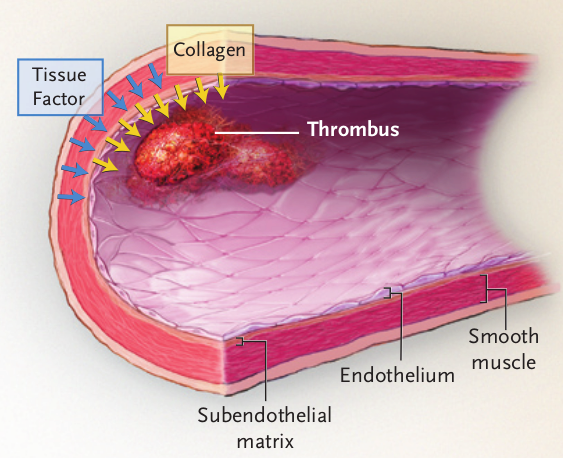
\includegraphics[width=0.35\textwidth]{Figures/Furie.png}
\caption{\label{sec:fur} Vessel wall showing the collagen and Tissue Factor locations (image from \citet{Furie:2008})}
\end{figure}

Historically the importance of the intrinsic pathway remained speculative because patients with factor XII (initial enzyme in the contact system) deficiency did not present bleeding disorders. Patients lacking of factor VII (initial enzyme in the extrinsic system) prompt bleeding disorders suggesting that the contact system had a minor role in haemostasis and therefore in thrombosis as well. It was not until the work of \citet{Renne:2005} that the importance of the contact system for thrombus formation was elucidated. Renne and co-workers showed that infusion of human factor XII into murine blood lacking of factor XII resulted in a restitution of thrombotic activity. This findings support even more that contact activation is crucial for thrombosis in biomedical devices because factor XII adheres to must of the materials used in prosthetic devices initiating thrombin formation.\\

Figure~\ref{sec:intrinsic_diagram} shows the intrinsic pathway including the three enzymatic reactions (auto-activation, auto-hydrolysis and reciprocal activation) that activate factor XII and begin the coagulation cascade. The intrinsic pathway initiates at the artificial surface where factor XII follows a surface mediated reaction to form factor XIIa (auto-activation). Also at the surface \nomenclature{\textbf{HMWK}}{High molecular weight kininogen}%
high molecular weight kininogen (HMWK) binds to prekallikrein \nomenclature{\textbf{PK}}{Prekallikrein}%
 (PK) and to factor XI. Once PK is bind to HMWK it transforms into \nomenclature{\textbf{Kal}}{Kallikrein}% 
Kallikrein (Kal). Activation of factor XII by Kal (reciprocal activation) and auto-hydrolysis of factor XII complete the three different mechanisms of factor XII activation. In addition Kal transforms factor XIIa to XIIf (fragmented) which serves as a regulator of factor XIIa. Activation of factor XI to XIa by the presence of factor XIIa mark the end of the contact system. The intrinsic system continues with the activation of factor IX to IXa by the action of factor XIa. Factor IXa forms a complex with calcium and VIIIa (which is activated by thrombin). Finally complex IXa$\backslash$VIIIa$\backslash$Ca activate factor X. The intrinsic and extrinsic pathways merge in the production of factor Xa. \\

\paragraph{\underline{Extrinsic system (pathway):}}
This pathway is triggered by the presence of \nomenclature{\textbf{TF}}{Tissue Factor}%
Tissue Factor (TF) which is present at the sub-endothelium (see Figure~\ref{sec:fur}). TF is also known as factor III or thromboplastin. When TF is exposed to blood flow, it binds to plasma factor VII to form the TF$\backslash$VII complex. TF$\backslash$VII complex promotes the activation of factor VII forming the complex TF$\backslash$VIIa. It is important to mention that pico-molar concentrations of VIIa circulate normally in the blood thus allowing, in the presence of TF, the direct formation of TF$\backslash$VIIa complex \citep{Gorbet:2004}. In the presence of calcium and phospholipids TF$\backslash$VIIa complex activate factor X, as pointed out before, here is where the intrinsic and extrinsic pathways come together. In addition TF$\backslash$VIIa complex can activate factor IX, hence communication between extrinsic and intrinsic systems take place. TF expression by monocytes was observed by \citet{Wilhelm:1998} and correlated to the presence of bio-materials boosting the extrinsic pathway. Figure~\ref{sec:extrinsic_diagram} shows a diagram of the extrinsic pathway.\\

\paragraph{\underline{Common pathway:}}
Factor Xa forms a complex with activated factor Va. In the presence of calcium complex Xa$\backslash$Va converts prothrombin into Thrombin which is the master regulation of coagulation. Thrombin cleaves activation peptides from Fibrinogen to form fibrin monomers that result into a clot at the site of the injury. It also activates factor XIII that gives mechanical structure to the fibrin clot. In addition thrombin activates platelets that adhere to the fibrin clot and seal it. In order to form an amplification feedback loop, thrombin activates factor V, factor XI and factor VIII. Figure~\ref{sec:coagcas_diagram} shows the coagulation cascade involving the three pathways previously mentioned.\footnote{A really good graphical effort from the Johns Hopkins University to explain the coagulation cascade can be found in \url{http://www.hopkinsmedicine.org/hematology/Coagulation.swf}}\\

\begin{figure}[h]
\tikzstyle{vspecies}=[rectangle, minimum size=0.5cm,draw=blue!80]{
	\begin{tikzpicture}[auto, outer sep=3pt, node distance=2.5cm,>=latex']
	\node [vspecies] (FXII) at (0,0) {$XII$};
	\node [vspecies] (FXI) at (3,0) {$XI/HMWK$};
	\node [vspecies] (PK) at (-3,0) {$PK/HMWK$};
	\node [vspecies] (FXIIa) at (0,-1.5) {$XII_{a}$};
	\node [vspecies] (FXIaHMWK) at (3,-3) {$XI_{a}/HMWK$};
	\node [vspecies] (Kal) at (-3,-3)  {$Kal/HMWK$};
	\node [vspecies, below of = FXIIa] (FXIIf) {$XII_{f}$};
	\node [vspecies] (FIX) at ( 6,-3 ) {$IX$};
	\node [vspecies, below of = FIX] (FIXa) {$IX_{a}$};	
	\node [vspecies, left of = FIXa] (Ca) {Ca};
	\node [vspecies, left of = Ca] (FVIIa) {$VIII_{a}$};
	\node [vspecies] (X) at ( 8 , -5.5 ) {$X$};
	\node [vspecies, below of = X] (Xa) {$X_{a}$};
	\draw [->,thick] (FXII) -- (FXIIa) ;
	\draw [->,thick] (PK) -- (Kal) ;
	\draw [->,thick] (FXI) -- (FXIaHMWK) ;
	\draw [-,thick] (0,-2.6) -| (0.8,-2.6) ;
	\draw [->,thick] (0.8,-2.6) |- (0.0,-0.75) ;
	\draw [->,thick] (-2.5,-2.6) |- (0,-0.75) ;
	\draw [->,thick] (FXIIa) -- (FXIIf) ;
	\draw [->,thick] (Kal) -- (0,-3) ;
	\draw [->,thick] (FXIIa) -- (3,-1.5) ;
	\draw [->,thick] (FIX) -- (FIXa) ;
	\draw [->,thick] (FXIaHMWK) |- (6,-4) ;
	\draw [->,thick] (X) -- (Xa) ;
	\draw[red,thick,dotted] ($(PK.north west)+(-0.4,0.3)$)  rectangle ($(FXI.south east)+(0.1,-0.2)$) ;
	\draw[green,thick,dotted] ($(FVIIa.north west)+(-0.4,0.3)$)  rectangle ($(FIXa.south east)+(0.1,-0.2)$);
	\coordinate [text = red,label=left:Artificial surface] (AS) at (-2,0.5);
	\coordinate [text = red,label=left:Complex] (VII_Ca_IX) at (1.5,-5.1);
	\draw [->,thick] (3.8,-6.1) |- (8,-6.5) ;
	\end{tikzpicture}}\\
	\caption{\label{sec:intrinsic_diagram} Intrinsic pathway based on the model presented by \cite{Chatterjee:2009a} and traditional biochemical theory.}
\end{figure}
%The model of~\citet{Chatterjee:2009a} does not considers the adsorption process of proteins over the foreign surface. When an artificial surface is present in the blood flow; proteins (albumin, fibrinogen, factor XII, HMWK, etc) rapidly adhere to the artificial surface. This protein layer changes dynamically in what is called the Vroman effect \cite{Vroman:1980}. This effect explains that the protein layer evolves due to protein competition to adsorb to the artificial surface and thus the production of factor XIIa will be influenced by the rate of absorption of factor XII. Once factor XII adheres to the surface it is activated due to the three enzymatic reactions previously mentioned. 
\begin{figure}[h]
\tikzstyle{vspecies}=[rectangle, minimum size=0.5cm,draw=blue!80]{
	\begin{tikzpicture}[auto, outer sep=3pt, node distance=2.5cm,>=latex']
	\node [vspecies] (TF) at (0,0) {TF (Vessel injury)};
	\node [vspecies] (FVII) at (2.5,-1.5) {$VII$};
	\node [vspecies, below of = TF] (TF/FVII)  {$ TF \backslash VII$};
	\node [vspecies, right of = FVII ] (FVIIa)  {$ VII_{a}$};
	\node [vspecies, below of = FVII] (TF/FVIIa)  {$ TF \backslash VII_{a}$};
	\node [vspecies, left of = TF/FVIIa] (Ca) {$Ca$};
    \node [vspecies, right of = TF/FVIIa] (X) {$X$};
	\node [vspecies, below of = X] (Xa) {$X_{a}$};
	\draw [->,thick] (TF) -- (TF/FVII);
	\draw [->,thick] (FVII) -- (TF/FVIIa);
	\draw [->,thick] (FVII) -- (0,-1.5);
	\draw [->,thick] (TF/FVII) |- (2.5,-2.5);
	\draw [->,thick] (FVIIa) |- (2.5,-3.0);
	\draw [->,thick] (X) -- (Xa);
	\draw[green,thick,dotted] ($(Ca.north west)+(-0.4,0.3)$)  rectangle ($(TF/FVIIa.south east)+(0.1,-0.2)$);
	\coordinate [text = red,label=left:Complex] (VII_Ca_IX) at (1.0,-3.6);
	\draw [->,thick] (1.5,- 4.7) |- (5.0,-5.5);
	\end{tikzpicture}}\\
	\caption{\label{sec:extrinsic_diagram} Extrinsic system pathway (sometimes refer as TF pathway).}
\end{figure}

\paragraph{\underline{Inhibitors of coagulation}}
The coagulation cascade has many feed back loops that amplify the production of thrombin. A counterpart that blocks the amplification loops is present in blood in order to reach haemostatic balance, hence clotting is active until vessel integrity is reached. The main inhibitors of coagulation are:
\begin{itemize}
\item \textbf{Protein C} is a vitamin K-dependent protein that inactivates factors Va and VIIIa.
\item \textbf{Antithrombin} neutralize factor Xa and Thrombin by forming a complex. It is also capable of inhibiting factors IXa, XIa and XIIa.
\item  \nomenclature{\textbf{TFPI}}{Tissue Factor pathway inhibitor}% 
\textbf{Tissue factor pathway inhibitor (TFPI)} is the main inhibitor of TF$\backslash$VIIa complex and factor Xa. TFPI is present on the lumminal surface of the vascular endothelium, also in platelets, monocytes and plasma.
\end{itemize}

\begin{figure}[h!]    
\tikzstyle{vspecies}=[rectangle, minimum size=0.5cm,draw=blue!80]{
	\begin{tikzpicture}[auto, outer sep=3pt, node distance=2.2cm,>=latex']
	\node [vspecies] (FXII) at (0,0) {$XII$};
	\node [vspecies] (FXI) at (2,0) {$XI \backslash HMWK$};
	\node [vspecies] (PK) at (-2,0) {$PK \backslash HMWK$};
    \node [vspecies] (TF) at (7,0) {TF (Vessel injury)};
	\node [vspecies] (FXIIa) at (0,-1.5) {$XII_{a}$};
	\node [vspecies] (FVII) at (9.5,-1.5) {$VII$};
	\node [vspecies, below of = TF] (TF/FVII)  {$ TF \backslash VII$};
	\node [vspecies, right of = FVII ] (FVIIa)  {$ VII_{a}$};
	\node [vspecies, below of = FVII] (TF/FVIIa)  {$ TF \backslash VII_{a}$};
	\node [vspecies, left of = TF/FVIIa] (Ca_2) {$Ca$};
	\node [vspecies] (FXIaHMWK) at (2,-2) {$XI_{a} \backslash HMWK$};
	\node [vspecies] (Kal) at (-2,-2)  {$Kal/HMWK$};
	\node [vspecies] (FXIIf) at (0.0, -3.2) {$XII_{f}$};
	\node [vspecies] (FIX) at ( 5,-2 ) {$IX$};
	\node [vspecies, below of = FIX] (FIXa) {$IX_{a}$};	
	\node [vspecies, left of = FIXa] (Ca) {$Ca$};
	\node [vspecies, left of = Ca] (FVIIIa) {$VIII_{a}$};
	\node [vspecies] (X) at ( 7 , -5.0 ) {$X$};
	\node [vspecies, below of = X] (Xa) {$X_{a}$};
	\node [vspecies, left of = Xa] (VA) {$V_{a}$};
	\node [vspecies, left of = VA] (V) {$V$};
	\node [vspecies, below of = Xa] (XA_VA) {$X_{a} \backslash V_{a}$};
	\node [vspecies, right of = XA_VA] (PTII) {Prothrombin};
	\node [vspecies, below of = PTII] (Thrombin) {Thrombin};
	\node [vspecies, right of = Thrombin] (Fibrinogen) {Fibrinogen};
	\node [vspecies, below of = Fibrinogen] (Fibrinm) {Fibrin m};
	\node [vspecies, below of = Fibrinm] (Fibrinp) {Fibrin p};
	\node [vspecies, below left of = Thrombin] (XIII) {$XIII$};
	\node [vspecies, below of = XIII] (XIIIa) {$XIIIa$};
	\node [vspecies, left of = XIII] (Plat) {Activated Platelets};
 	\node [vspecies, above of = Plat] (Plats) {Platelets};
 	\node [vspecies, below of = Fibrinp] (Sfibrin) {Stable fibrin};
	\draw [->,thick] (FXII) -- (FXIIa) ;
	\draw [->,thick] (PK) -- (Kal) ;
	\draw [->,thick] (FXI) -- (FXIaHMWK) ;
	\draw [-,thick] (0.0,-2.3) -- (0.7,-2.3) ;
	\draw [->,thick] (0.7,-2.3) |- (0.0,-0.75) ;
	\draw [->,thick] (-1.5,-1.6) |- (0,-0.75) ;
	\draw [->,thick] (FXIIa) -- (FXIIf) ;
	\draw [->,thick] (Kal) |- (0,-2.5) ;
	\draw [->,thick] (0.55,-1.5) -- (1.8,-1.5) ;
	\draw [->,thick] (FIX) -- (FIXa) ;
	\draw [->,thick] (FXIaHMWK) |- (5,-3.0) ;
	\draw [->,thick] (6.5,-3.3) -- (5.0,-3.3) ; 
	\draw [->,thick] (X) -- (Xa) ;
	\draw [->,thick] (3.0,-4.8) |- (7,-6.3) ;
	\draw [->,thick] (TF) -- (TF/FVII);
	\draw [->,thick] (FVII) -- (TF/FVIIa);
	\draw [->,thick] (FVII) -- (7.0,-1.5);
	\draw [->,thick] (TF/FVII) -- (9.5,-2.2);
	\draw [->,thick] (FVIIa) |- (9.5,-2.7);
	\draw [->,thick] (8.5,- 4.3) |- (7,-6.0);
	\draw [->,thick] (Xa) -- (XA_VA);
	\draw [->,thick] (VA) |- (7,-8.0);
	\draw [->,thick] (V) -- (VA);
	\draw [->,thick] (PTII) -- (Thrombin);
	\draw [->,thick] (XA_VA) |- (9.2,-10.5);
	\draw [->,thick] (XIII) -- (XIIIa);
	\draw [->,thick] (Fibrinogen) -- (Fibrinm);
	\draw [->,thick] (Fibrinm) -- (Fibrinp);
	\draw [->,thick] (Fibrinp) -- (Sfibrin);
	\draw [->,thick,red] (Thrombin) -- (5.5,-11.45);
	\draw [-,thick,red,dashed] (8.7,-11.2) |- (3.5,-10.3);
	\draw [->,thick,red,dashed] (3.5,-10.3) |- (3.5,- 7.4);
	%\draw [-,thick,red,dashed] (3.5,-10.3) -| (1.75,-1.8);
	\draw [->,thick,red,dashed] (3.8,-10.3) |- (2.2,-1.5);
	\draw [-,thick,red,dashed] (8.9,-11.2) |- (6.3,-10.0);
	\draw [->,thick,red,dashed] (6.3,-10.0) |- (5.2,-3.5);
	\draw [->,thick] (Plats) -- (Plat);
	\draw [->,thick] (Plat) |- (11.3,-17.3);
	\draw [->,thick,red] (9.5,-12.0) |- (11.3,-13.0);
	\draw [->,thick] (XIIIa) |- (11.3,-17.0);
	\draw [->,thick,red] (Thrombin) |- (7.7,-14.0);
	\draw[green,thick,dotted] ($(Ca_2.north west)+(-0.4,0.3)$)  rectangle ($(TF/FVIIa.south east)+(0.1,-0.2)$);
	\coordinate [text = red,label=left:Complex] (VII_Ca_IX) at (8.2,-3.3);
	\draw[red,thick,dotted] ($(PK.north west)+(-0.4,0.3)$)  rectangle ($(FXI.south east)+(0.1,-0.2)$) ;
	\draw[green,thick,dotted] ($(FVIIIa.north west)+(-0.4,0.3)$)  rectangle ($(FIXa.south east)+(0.1,-0.2)$);
	\coordinate [text = red,label=left:Artificial surface] (AS) at (-1.0,0.5);
	\coordinate [text = red,label=left:Complex] (VII_Ca_IX) at (1.5,-3.8);
	\end{tikzpicture}}\\
	\caption{\label{sec:coagcas_diagram} Blood-coagulation cascade (intrinsic, extrinsic and common pathways) and fibrin production.}
\end{figure}

\subsubsection{Vromman effect}
An adsorption process of proteins over the foreign surface takes places during the first instants of blood contacting a biomedical device. When an artificial surface is present in the blood flow; some proteins like albumin, fibrinogen, factor XII or HMWK rapidly adhere to it. This protein layer changes dynamically in what is called the Vroman effect \citet{Vroman:1980}. Vroman and co-workers observed the replacement of fibrinogen in an attempt to identify the adhesion pathway of proteins over artificial surfaces. The process that was used to track the proteins revealed an alteration in the fibrinogen deposited onto the surface. HMWK apparition and fibrinogen disappearance was observed when fibrinogen was deposited onto hydrophilic glass-like surfaces and put in contact with plasma. Fibrinogen alteration was clear when HMWK deficient plasma was used and the deposited fibrinogen remain unaltered. This event suggest that HMWK and fibrinogen compete dynamically for binding sites. In whole blood proteins compete to adsorb in free sites of the artificial surface. In particular the rate of factor XII adsorption will directly influence the initiation of the intrinsic system as it was previously explained. 

\subsubsection{Platelets}
Normally non-activated platelets circulate in the blood flow and they become active in the first instants of haemostasis (in what is call primary haemostasis). Platelets are recruited to the injury and promote coagulation reactions. They also seal the fibrin clot and therefore platelets become a major component of the thrombus. Activation of platelets occurs when they contact any type of thrombogenic surface. They provide a fundamental base in which reactions of coagulation can take place (we had referred to this base as a phospholipid surface). There exist two pathways to platelet activation \citep{Furie:2008}. One pathway is due to the interactions of von Willebrand factor (vWF) and glycoprotein VI with collagen; this pathway is independent of thrombin and its result is the adhesion of platelets to the injury. A second pathway is related to thrombin that activates platelets directly and also produces serotonin and thromboxane $A_{2}$ that amplify platelet activation. In addition platelets can be mechanically activated by the flow. \citet{Hellums:1994} identify a shear stress threshold for platelet activation that depend on the stress magnitude and the exposure time.\\
\paragraph{\underline{Platelet activation due to medical devices}}
Platelet activation has been observed in several clinical procedures and bio-mechanical devices due to high shear stress. Once activated platelets increase their adhesive properties. In vivo the bouncing off or adhesion of platelets to the thrombus is regulated by the interaction of GPIIb$\backslash$IIIa complex with fibrinogen and by the interaction of GPIIb$\backslash$IIa complex with vWF. However, for in vitro cases the Vroman effect takes place and a protein film is formed over the artificial surface. Fibrinogen which is in the protein film has a strong affinity with platelets. Platelets adhere to fibrinogen and promote the contact activation system as observed in \cite{Renne:2005}. 
\subsubsection{Complement system}
The complement system allows antibodies to kill bacteria. This activity was said to "complement" the antibacterial activity of the antibody and hence the name. It has fundamental clinical implications in the context of life-threatening tissue injury and inflammation. Complement system is structured by the classical and the alternative pathways see Figure~\ref{diag:complement}. The classical pathway is triggered by antigen-antibody complexes while the alternative pathway is activated by contact activation of foreign surfaces such as fungal, bacterial polyssaccharides, lipopolysaccharides, particles and \textbf{bio-material surfaces}.\\

\begin{figure}[h]
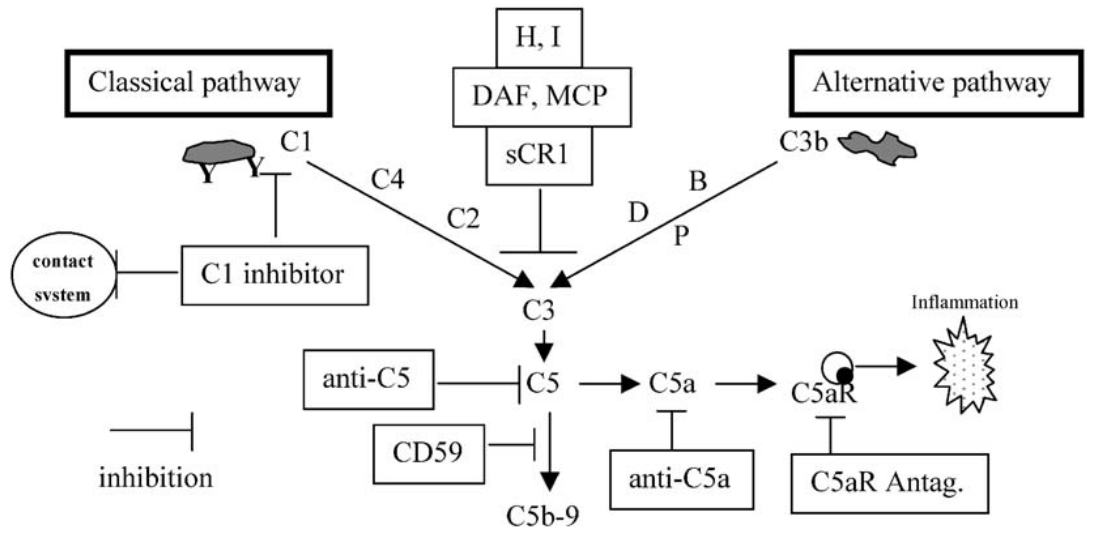
\includegraphics[width=0.6\textwidth]{Figures/contactsystem.png}
\caption{\label{diag:complement} Complement system diagram from \cite{Gorbet:2004} (Kirschfink M)}
\end{figure}
The coagulation cascade is related to the complement system at several levels. Thrombin and coagulation factors XIa, Xa, IXa and plasmin were all found to effectively cleave C3 and C5 molecules which are central components of the complement system. Furthermore the contact system relates directly to the factors that initiate the complement system.  In Table~\ref{tab:comple} all the interactions of the complement system with the coagulation systems are shown.\\
\begin{table}[h]
\begin{tabular}{l l}
\hline
Protein & Type of interaction \\
\hline
Thrombin & Proteolysis of C3, C5, C6 and factor B\\
Factor XIIa & Proteolysis of C1r, C1s and C3\\
Kallikrein & Proteolysis of C1, C5 and Factor B \\
Antithrombin III & Protect RBC form lysis by mC5b-9\\
Bb & Proteolysis of prothrombin \\
C3bBb & Proteolysis of prothrombin \\
C1 inhibitor & Inactivates FXIIa and kallikrein \\
S protein (vitronectin) & Stabilizes plasminogen activator inhibitor 1 \\
C4b-binding protein & Binds to the vitamin K-dependant protein S \\
\hline
\end{tabular}
\caption{\label{tab:comple}Interactions between complement and coagulation systems \cite{Gorbet:2004}}
\end{table}
\paragraph{\underline{Effect of biomedical devices in the Complement system:}}
\citet{Gorbet:2004} pointed out the importance of complement system interaction with the coagulation process when artificial surfaces are present. In particular an inflammatory response is observed in the presence of bio-materials. This inflammation is due to the activation of the alternative pathway. In addition the increase activity of the complement system may increase leukocyte TF expression and therefore thrombin production.
\subsubsection{Leukocytes}
Several types of leukocytes are present in blood. Neutrophils, monocytes, lymphocytes, basophils and eosinophils are the main five types of leukocytes that form the immune system. Artificial surfaces interaction with Neutrophils($40-60 \%$ of leukocytes population) and monocytes ($5 \%$ of leukocyte population) may activate this type of cells. One of the most important effects of leukocyte activation to thrombosis is the expression and synthesis of TF. Leukocyte adhesion may also participate in inflammation and therefore promoting a feedback loop with the contact system.\\

\subsubsection{Blood flow influence in thrombosis}
Blood flow enhances the transport of coagulation factors to the surface (vessel wall injury or the artificial surface). The rate of transport (diffusive and convective) is extremely important for coagulation biochemistry. Observing the characteristic time scales of enzymatic reactions, convective and diffusive transport can enhance a deeper understanding of each component of the haemostastic system as pointed out by \citet{Rana:2016}.    
%When it comes to the extrinsic pathway, it is found that for high shear rates the activation of factor Xa by the complex TF$\backslash$VIIa increases. 
\citet{Basmadjian:1997} showed the relation between the artificial surface reactivity and the flow. At low flow rates, activation rates of Factor IX (intrinsic system) are high and do not depend on  the surface reactivity. However, as the flow shear rate increases, the activation of factor IX depends a lot on the surface reactivity. This findings are really interesting because even when the activation rate of Factor XII is close to zero (almost anti-thrombogenic surface), the activation of factor IX continues. This supports the fact that the best way to design non-thrombogenic surfaces is to include both the reactivity of the tissue and the characteristics of the flow.\\
A clear influence of the flow in platelet activation, aggregation and adhesion is present \citep{Hellums:1994,Turitto:1975,Grabowski:1972}. Fluid mechanical shear stress can be pictured as a platelet agonist that will increase binding affinity between the different platelet agonists. Furthermore a clear interaction of platelet activation and shear stress has been observed at some particular threshold \nomenclature{\textbf{SS}}{shear stress}%
shear stress (SS) levels. Measurable changes in the platelet response are seen when the thresholds of SS are reached, these thresholds depending strongly on the time of exposure. Figure~\ref{diag:ssthreshold} shows the dependency of the platelet serotonin release (activation of platelets) to the shear stress and the exposure time. In particular a key event of the stress-induce activation and aggregation is the binding of vWF to platelet membrane glycoprotein Ib. Grabowski \textit{et al.} \citep{Grabowski:1972} demonstrated that increasing shear rate may increase the flux of platelets to a foreign surface not only by diminishing the thickness of the platelet concentration boundary layer but also by simultaneously augmenting the platelet diffusion coefficient; a dependency of the platelet adhesion to shear rate is therefore present.\\

In addition thrombus architecture is greatly influenced by how the fibrin plug and platelets adhere to thrombogenic surface, therefore the characteristics of the flow like wall shear or turbulence are extremely important to understand the dynamic process of thrombus formation.\\

\begin{figure}[h]
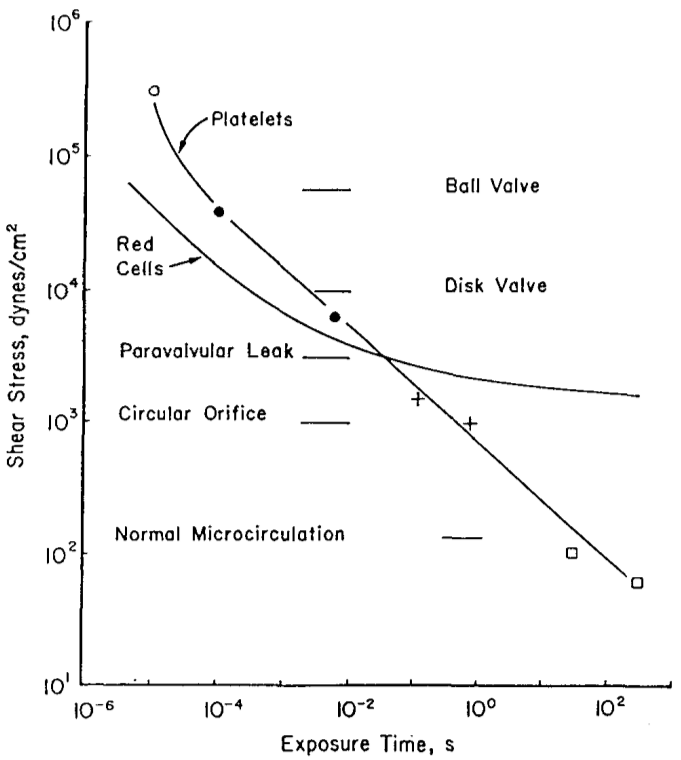
\includegraphics[width=0.3\textwidth]{Figures/hellums_threshold}
\caption{\label{diag:ssthreshold}}
\end{figure}
Similar studies as for platelets have been done in order to evaluate the influence of the flow on leukocyte adhesion, suggesting an important connection; however a bigger effort needs to be done. Finally, turbulence may have an effect on the recirculation zones that result in hemolysis and cell activation but its influence in thrombus growth is poorly understood and research is still on going.

\subsubsection{Virchow's triad and coagulation tests}
There are several test and criteria that allow us to test the risk of thrombosis from a biomedical device. For instance Virchow's triad consist of three risk elements that build a criteria for venous thrombosis.
Virchow's components are: 
\begin{itemize}
\item Slowing down of the local blood flow
\item Hypercoagulatibity of the blood
\item Vessel damage
\end{itemize}
Assessment of the biomedical devices needs to be performed in order to test the thrombogenicity. This test vary according the device and procedure in which the device will be use. In Table~\ref{tab:Thrombogenicity} several examples of device testing are presented.
\begin{table}[h]
\begin{tabular}{c p{4.5cm}}
\hline
\textbf{Device} &  \textbf{Test}\\
\hline
Intervention Catheters & 4 hour canine NAVI study\\
Indewelling Catheters & 30 day animal study with platelet activation and leukocyte information\\
Stents-Grafts & Large animal studies\\
VADs & Large animal studies\\
Bypass circuit components & In vitro coagulation assays \\
\hline
\end{tabular}
\caption{\label{tab:Thrombogenicity} Thrombogenicity testing from the FDA for several biomedical devices}
\end{table} 
\subsubsection{Conclusion}
\subsection{\label{sec:mechanical}Thrombosis Modelling}
The modelling of thrombosis can easily turn into complicated mathematical models, therefore an isolated analysis of each component of thrombosis may be easier and more clear to present. In this section the state of the art in thrombosis modelling is presented paying closed attention to the multi-physic nature of the problem.
\subsubsection{Biochemistry of intrinsic, extrinsic and common pathways}
One of the first models of thrombin generation was presented by Jones and Mann \citep{Jones:1994}. This model simulates the TF pathway (extrinsic pathway) including 18 species and 20 differential equations that describe the coagulation reactions. The model is solved using a Runge-Kutta integration technique.\\
A specific model of the intrinsic and common pathways was presented by \citet{Gregory:1994}. The model is comprised of 20 dominant reactions with 11 components that can be reduce to 4 coupled ODEs with Leveque's regime hypothesis. A polynomial algebraic equation can be obtained and 3 steady state concentrations for coagulants are analysed. The central coagulant in this model is Factor XII which was considered in 3 states (activated, bind to the surface and fragmented).\\
Another model of the intrinsic pathway was developed by \citet{Zarnitsina:1996}. In  this model 8 differential equations account for the activation of factors XI, IX, X, II, I, VIII, V protein C. Tenase and prothrombinase complex are calculated as a function of calcium concentration. The model assumes a constant flux at the injury site of activated factor XI.\\ 
\citet{Kuharsky:2001} developed a physical and chemical model that accounts for  platelet and coagulation events that occur in a thin layer, called the reaction zone, just above a small vascular injury. The KF model takes into account the plasma-phase, subendothelial-bound and platelet-bound enzymes and zymogens as well as activated and unactivated platelets. All species in the reaction zone are assumed to be well mixed; each species is characterized by its concentration that is tracked in time using an ordinary differential equation. Advective and diffusive transport of fluid-phase species (chemicals and platelets) into or out of the reaction zone is modelled by a mass-transfer term in which the mass-transfer coefficient depends on flow and diffusion parameters. The disadvantage of this model is the poor treatment of the flow.\\
In the work of Xu \textit{et al.} \cite{Xu:2008} a two dimensional model is presented where a macroscopic view of the flow is described by the NS equations. However, for the for the microscale interactions between the platelets and coagulation reactions, an extended stochastic discrete model was used.\\
Anand \textit{et al.} \citep{Anand:2003, Anand:2006, Anand:2008} biochemical reactions and rheological aspects are taken into account, in addition of reactions for the production of fibrin. The model of Anand \citep{Anand:2003} was used in a simplified way by Bodn\'{a}r and Sequeira \citep{Bodnar:2008} to study the clot formation and growth of thrombus in the vicinity of an injured vessel wall.\\
A mathematical model for the contact activation of factor XII by a pro-coagulant surface was developed by Guo \textit{et al.} \citep{Guo:2006}. The model of Guo uses a Michaelis-Menten kinetic mechanism simplifying the coagulation cascade of enzymatic reactions in a single enzymatic reaction. Therefore the model can be divided in two steps; first the activation of FXIIa as function of a catalytic surface potential (that variates according to the water-weattability of the surface) is calculated and then FXIIa interacts with the rest of the cascade of reactions in the form of a substrate. These two steps are combined to predict the coagulation time. Guo concludes that the material induced coagulation is a surface mediated event thus the coagulation times depends strongly on the surface area and the properties of the surface. Finally the results suggest that procoagulant surfaces have no influence in enzymatic reactions other than FXII activation
\subsubsection{Platelet activation and adhesion}
Sorensen \textit{et al.} \citep{Sorensen:1999} developed a two dimensional model of a coupled set of convection-diffusion-reaction equations, which attempts to simulate platelet-platelet and platelet-surface adhesion as well as platelet activation by relevant agonist (RP, AP, $a_{pr}$, $a_{ps}$). The model also accounts for platelet-phospholipid-dependent thrombin generation and thrombin inhibition by antithrombin III. The velocity fields come from the well know Poiseuille solution.\\ 
\citet{Mandrusov:1998} studied the Vroman effect in a shear flow chamber for a mixture of plasma and saline solution. Experiments were compared against numerical simulations to study the kinetics of plasma protein deposition. A band of fibrinogen moving downstream was observed and calculated. This band promotes platelet adhesion that was also observed in the experiments. A single-component unsteady convective-diffusion equation was solved for a two dimensional  domain. Deposition of fibrinogen and HMWK was calculated at the wall using the composition of the species. Natural convection had a great effect in the experiments, therefore, the experimental and numerical results showed important differences.\\
Fogelson and Guy \citep{Fogelson:2004} presented a model that account for platelet adhesion in an injured vessel using distributions of elastic links which generate stresses that influenced the fluid motion. This method is interested at the microscale of platelets events and considers the wall and the flow as a continuum.\\
A backward-facing step (BFS) configuration was studied by \citet{Taylor:2014}. In this work thrombus growth is investigated using an magnetic resonance imaging (MRI). The acrylic BFS configuration is connected to a pump in a closed loop in which bovine blood circulate for 90 minutes. Several MRI were performed to capture the thrombus growth and then simulations were performed with the segmentation geometry. The simulations where performed at a Reynolds number of 490 and the wall shear stress distribution over the thrombus was calculated observing a clear dependence on the thrombus topology. In an posterior work \citet{Taylor:2015} used a simplified form the model of Fogelson and Guy\citep{Fogelson:2004}. A modified Brinkman term was added to the equations in order to account for thrombus growth; This term act as a momentum sink in regions with a high concentration of platelet-platelet links. The advantage of this treatment is that it allows to keep the original mesh.\\
\subsubsection{Thrombus growth}
Goodman \textit{et al.} \citep{Goodman:2005} present a model in which thrombus growth is handled by increasing the viscosity in mesh cells where the volume of adherent platelets was grater than the volume of the grid. This model also takes into account embolization, platelet adhesion and platelet activation. Transport properties were taken as in \citep{Wootton:2002}. The model does not account for protein absorption it assumes proteins at the surface are in equilibrium. Finally the model of \citet{Goodman:2005} is compared with experimental results showing a good agreement for the thrombus growth.\\
Leiderman and Folgelson \citep{Leiderman:2011} present an extension of the Kuharsky and Fogelson \citep{Kuharsky:2001} model that incorporates spatial variations and explicitly models the growth of a thrombus and how this is coupled with the local fluid dynamics; the platelet adhesion is model as in \citet{Fogelson:2004}.\\

\subsubsection{Thrombosis risk assessment in biomedical devices}
Biasetti \textit{et al.} \citep{Biasetti:2011} studied an unsteady blood flow in aneurysmatic aortas using a Newtonian and a non newtonian model for the blood using the $\lambda_{2}$ criteria for vortex-eduction. Then a possible relation between vortex and intraluminal thrombus (ILT) formation was investigated. In a posteriori work Biasetti \textit{et al.} \citep{Biasetti:2012} present a model in which biochemical reaction were added with a set of convection-diffusion-reaction equations from \citep{Jones:1994}. The results showed a big influence of the flow (shear rates and vortex) on the production of thrombin and the ILT growth.\\
In contrast, Achille \textit{et al.} \citep{Achille:2014} presented a predictor of intraluminal thrombus formation in abdominal aortic aneurysms using a chemistry-free approach. It mimics the platelets activation due to flow-induce shear and platelet adhesion at the walls where the haemodynamic activity is favourable (recirculation zones). Achille \textit{et al.} applied the model to 10 carotid arteries and 6 abdominal aortic aneurysms from which half of them where healthy. The results show an impressive effectiveness of the predictor; however more studies have to be done to include nascent thrombus that were not include in the study and that are crucial for medical practice.\\

\subsubsection{Conclusion}
Thrombosis modelling efforts are focused to predict thrombus growth in vivo. In general a good amount of work has been dedicated to model extrinsic and common pathways. As well literature can be found on platelet activation, aggregation. Porosity in the thrombus has also been studied by the used of a Birkman term. On the other hand many other factors relevant to thrombosis in biomedical devices lack of a mathematical model like the contact system, platelet magration to the wall, effect of turbulent flows and the influence of the inflammation process (complement system and leukocyte activity). 

\pagebreak
\subsection{A mathematical model for thrombosis in medical devices}
\subsubsection{Thrombosis block diagram}
In order to have a graphical representation of the mathematical modelling of thrombosis a diagram of thrombosis is presented with the inputs, outputs and processes involved. \\
 
\tikzstyle{block} = [draw, rectangle, minimum height=2.5em, minimum width=4em, node distance=2.5cm]
\tikzstyle{sum} = [draw, circle, node distance=1.5cm]
\tikzstyle{input} = [coordinate, node distance = 1.7 cm]
\tikzstyle{output} = [coordinate]
\tikzstyle{pinstyle} = [pin edge={to-,thin,black}]
\begin{tikzpicture}[auto, node distance=2cm,>=latex']
     We start by placing the blocks
    \node [input, name=input] {};
    \node [block, right of=input] (PAAB) {PAAB};
    \node [sum, right of=PAAB] (sum1) {};
    \node [sum, right of=sum1] (sum2) {};
    \node [block, right of=sum2] (EP) {EP};
    \node [input, name=in_TF, above of=sum2] {};
    \node [sum, right of=EP] (sum3) {};
    \node [sum, below of=EP] (sum4) {};
    \node [block, below of=sum4] (FPA) {FPA};
    \node [block, right of=sum3] (CP) {CP};
    \node [block, right of=CP] (FB) {FB};
    \node [block, above of=EP] (IP) {IP};
    \node [block, left of=IP] (AP) {CA};
    \node [input, name=in_intrinsic, left of=AP] {}; 
    \node [output, right of=FB] (output) {};
    %%%%%%%%%%%%%%%%%%%%%%%%%%%%%%%%ARROWS
    \draw [draw,->] (input) -- node {$X_{p}$} (PAAB);
    \draw [->] (PAAB) -- node {$y_{ps}$} (sum1);
    \draw [->] (sum1) -- node {$y_{ps}$} (sum2);
    \draw [->] (sum2) -- node [name=y1] {$y_T$}(EP);
    \draw [->] (in_TF) -- node [name=x_tf] [pos=0.99] {$+$} node [near start] {$X_{TF}$} (sum2);
    \draw [->] (EP) -- node [name=y2] {$y_{FX}$}(sum3);
    \draw [->] (sum3) -- node [name=y3] {$y_{TX}$}(CP);
    \draw [->] (CP) -- node [name=th] {$y_{th}$} (FB);
    \draw [->] (FB) -- node [name=y4] {$Y_{cs}$}(output);
    \draw [->] (th) |- (sum4);
    \draw [->] (sum4) -| node[pos=0.99] {$+$} 
        node [near end] {$y_{at}$} (sum2);
    \draw [->] (y4) |- (FPA);
    \draw [->] (FPA) -| node[pos=0.99] {$+$} 
        node [near end] {$y_{ps}$} (sum1);
    \draw [draw,->] (in_intrinsic) -- node {$X_{FXII}$} (AP);
    \draw [->] (AP) -- node [name=th] {$y_{th}$} (IP);
    \draw [->] (IP) -| node[pos=0.99] {$+$} 
        node [near end] {$y_{FX}$} (sum3);
\end{tikzpicture}

\begin{table}[h]
\begin{tabular}{c c}
\hline
Process & Meaning   \\
\hline
PAAB & Platelet Activation Aggregation and Binding \\
EP & Extrinsic Pathway \\
AA & Adsorption and activation of factor XII \\ 
IP & Intrinsic Pathway \\
CP & Common Pathway \\
FB & Fibrinolysis \\ 
FPA & Feedback Platelet Activation by Thrombin \\
\hline
\end{tabular}
\caption{\label{tab:process} Principal process of clot formation diagram }
\end{table}
\begin{table}[h]
\begin{tabular}{c c}
\hline
Inputs & Meaning   \\
\hline
$X_{FXII}$ & Concentration of Factor XII in blood \\
$S$ & Artificial Surface \\
$K_{m}$ & Michaelis-Menten constant \\
$X_{p}$ & Platelet concentration in blood \\
$D_{i}$ & Diffusion coefficients \\
$C_{i}$ & Concentration of species (Platelets or coagulation enzymes and complex) \\
$k_{i}$ & Reaction rate \\
$X_{TF}$ & Concentration of Tissue Factor (at the surface and in the blood stream) \\
\hline
\end{tabular}
\caption{\label{tab:process} Principal inputs of clot formation diagram}
\end{table}
\begin{table}[h]
\begin{tabular}{c c}
\hline
Outputs & Meaning   \\
\hline
$y_{ps}$ & Phospholipid surface (activated platelet concentration at the surface) \\
$y_{at}$ & Activated platelet by thrombin concentration at the surface \\
$y_T$ & Total activated platelet concentration at the surface \\
$y_{FX}$ & Concentration of $FX$ \\
$y_{TX}$ & Total concentration of $FX$ \\
$y_{th}$ & Thrombin concentration (at the surface and in the blood stream) \\
$Y_{cs}$ & Final output clot surface \\
\hline
\end{tabular}
\caption{\label{tab:process} Principal outputs of clot formation diagram}
\end{table}

\begin{table}[h]
\begin{tabular}{|p{5 cm} | p{3.5cm} | p{9.5 cm} |}
\hline
Article & Process & Summary\\
\hline
\citet{Jones:1994} & EP, CP & Phospolipid excess considered. \\
\hline
\citet{Chatterjee:2010} & AA, IP, EP, CP & Transport due to the flow are not taken into account. Influence of different plasma donors is shown.\\
\hline
\citet{Guo:2006} & AA, IP, EP, CP & Properties of the surface taken into account. Coagulation cascade reactions are taken as a single Michaelis-Menten reaction.\\
\hline
\citet{Kogan:2001} & AA, IP, EP, CP & Transport due to the flow are not taken into account.\\
\hline
\citet{Zarnitsina:1996} & IP, EP, CP & Constant concentration of activated factor XI as input.\\
\hline
\citet{Gregory:1994} & CA, IP & L\'{e}veque transport regime. FXII (binded to the wall) considered constant and equal to saturation level. HMWK considered as activated. All PK is complexed with HMWK.\\ 
\hline
\citet{Mandrusov:1998} & (Vroman effect protein adsorption model) & Transient Leveque problem accounting for Fibrinogen and HMWK deposition (Vroman effect)\\
\hline
\citet{Sorensen:1999} & PAAB,EP,CP,FB,FPA & Model focus in describing platelet dynamics (activated, adhere and resting) EP and CP simplified (only Thrombin, ATII and FII are accounted)\\
\hline
\citet{Kuharsky:2001} & PAAB, EP, CP & L\'{e}veque transport regime. Platelets as pro-coagulant surfaces. \\
\hline
\citet{Xu:2008} & PAAB, EP, CP, FB & NS for the flow. PAAB does not communicate with EP or FB. Clot interface tracked. \\
\hline
Anand \textit{et al.} \citep{Anand:2003, Anand:2006, Anand:2008} & EP, CP, PAAB, FB & Shear-thinning visco-elastic fluid. Platelet activation by thrombin, and by shear stress criteria. Constitutive model for the clot. Clott growth and dissolution. \\
\hline
\citet{Bodnar:2008} & EP,CP,FB & Clot growth with a viscosity constitutive law. Simplification of Anand \textit{et al.} model \\
\hline
\citet{Fogelson:2004} & PAAB & Model for platelet wall interaction (adhesion and aggregation) \\
\hline
\citet{Wootton:2002} &  PAAB, EP, CP, FB & Wall shear stress is correlated with lysis rate of mural thrombi\\
\hline
\citet{Goodman:2005} & PAAB, EP, CP, FB & 3D simulation of a conduct with variable cross section, platelet transport, adhesion and shear activation are taken into account. Thrombin production, emboli and thrombus growth are calculated and compared against experimental values\\
\hline
\citet{Biasetti:2012} & EP, CP  & Study the effect of flow transport in coagulation (in vivo) ussing the model of \cite{Jones:1994}\\
\hline
\citet{Leiderman:2011} & PAAB, EP, CP, FB, FPA & Two way communication between the growing thrombus and the flow. The porus nature of the clott is taking into account.\\
\hline
\citet{Taylor:2015} & PAAB, FB & BFS incompressible NS for a laminar configuration, the model uses a simplified version of \citet{Fogelson:2004} including a Brinkman term to account for thrombus growth \\
\hline
\end{tabular}\caption{\label{tab:recap}Summary of models presenting relating them with the block diagram}
\end{table}

As we can see from Table\ref{tab:recap} most of the models are focused on the extrinsic and common pathways thrombosis. Very few articles study thrombosis due to an artificial surface or in other words the intrinsic pathways. In addition complex flow configurations (which is the real case for biomedical devices) and activation of factor XII are not considered in the articles that study the intrinsic pathway \citep{Gregory:1994,Zarnitsina:1996,Mandrusov:1998,Chatterjee:2010,Kogan:2001}.\\ The role of turbulence and pulsate flows in platelet dynamics and coagulation pathways as well as the leukocyte expression of tissue factor and the complement system interactions with the coagulation cascade remain to be elucidated. In the next section two models to account for protein adsorption dynamics will be presented.
\subsection{Mathematical model for contact activation in blood flows}
A simulation of the contact system biochemical reactions immersed in a blood flow remains absent in the literature. Most of the models consider a source of activated factor IXa or a posterior activated factor. In order to investigate the contact pathway initiation in realistic flow regimes a kinetic enzymatic mechanism of factor XII activation can be couple in the form of a convection diffusion reaction equation communicating with the Navier Stokes equations.\\
\subsubsection{Convection diffusion reaction model}
One of the most common techniques to model thrombosis is the convection diffusion reaction model. This type of model considers a reaction network that is transported by a fluid in the form of diffusion and convection that yields to the following equation. 
\begin{equation}\label{eq:CDR}
\frac{\partial C_{i}}{\partial t} + \nabla \cdot (C_{i}u)  = \nabla \cdot (D_{i} \nabla C_{i}) + R_{i}
\end{equation}
Where: \\
$C_{i} : $ Concentration of i species \\
$D_{i} : $ Diffusion coefficient \\
$R_{i} : $ Source or sinks of species i \\
The source terms are obtained from a enzymatic kinetic scheme. Then initial conditions of the species concentrations are given as an input (free flow concentrations or wall concentrations in the case of Factor XII). As we can see from equation~\ref{eq:CDR} the diffusion coefficients and the velocity field are as well inputs in the model. In our case the Navier-Stokes equations for an incompressible fluid are solved to calculate the velocity fields.\\
A kinetic scheme of the intrinsic pathway can be used to investigate possible effects in the coagulation cascade due to the transport of enzymes. Two models for the activation of factor XII are presented. The first kinetical scheme was presented by \citet{Guo:2006} in which the catalytic potential is taken into account depending on the surface properties. A second scheme is taken from \citet{Chatterjee:2010} in which activation of factor XII is inhibited by two anti-thrombogenic enzymes  and a relations with the complement system are also present.
\subsubsection{Activation of Factor XII}
Up to date it is accepted that there are three enzymatic events that conduct to factor XII activation (auto-activation, auto-hydrolysis  and reciprocal activation of factor XII) as it is shown in figure~\ref{fig:activationFXIIa}.\\

\begin{figure}[h]
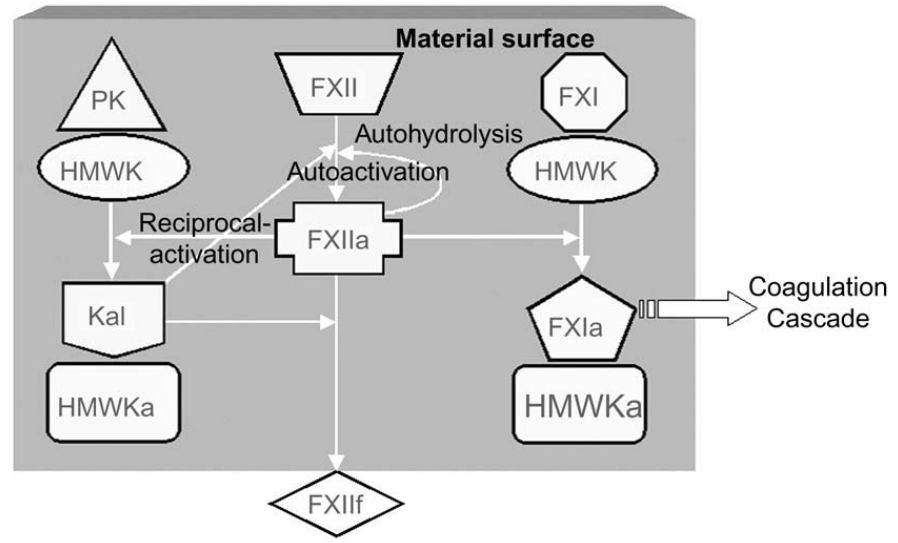
\includegraphics[scale=0.4]{Figures/ActivationFXIIa.png}
\caption{\label{fig:activationFXIIa} Enzymatic reactions for activation of  factor XII from \citet{Chatterjee:2009a}}
\end{figure}
The model of Chatterjee was used to predict the thrombin production time of a quiescent blood sample in the absence of tissue factor. The model propose that the main mechanism for thrombin formation is activation of factor XII. If only the contact system was taken into account the model would include the reactions in Table~\ref{Tab:Sourceterms}.\\
\begin{table}[h]
\begin{tabular}{p{7 cm} p{3 cm} p{3 cm} p{3 cm}}
\hline
Reaction & $M^{-1}s^{-1}$ & $s^{-1}$ & $s^{-1}$ \\
\hline
$XII \rightarrow XII_{a}$ &   & $k_{1} = 5.0 \times 10^{-4} $ & \\
$XII_{a} + XII \leftrightarrow XII_{a} / XII \rightarrow XII_{a} + XII_{a}$ & $k_{2} = 1 \times 10^{8}$  & $k_{3} = 750$ & $k_{4} = 3.3 \times 10^{-2}$  \\
$XII_{a} + PK \leftrightarrow XII_{a}/PK \rightarrow XII_{a} + K $ & $k_{5} = 1 \times 10^{8}$  & $k_{6} = 3.6 \times 10^{3} $  & $k_{7} = 40$ \\
$XII + K \leftrightarrow XII/K \rightarrow XII_{a} + K$ & $k_{8} = 1 \times 10^{8}$ & $k_{9} = 45.3$ & $k_{10} = 5.7$ \\
$PK + K \rightarrow K + K$ &$k_{11} = 2.7 \times 10^{4}$ &   &  \\
$K \rightarrow K.Inhibited $ & $ $ & $k_{12}=1.1 \times 10^{-2}$  & \\
$XII_{a} + CTI \leftrightarrow XII_{a}/CTI $ & $k_{13} = 1 \times 10^{8}$& $k_{14}=2.4$   & \\
$XII_{a} + C1_{inh}\rightarrow XII_{a}/C1_{inh} $ & $k_{15} = 3.6 \times 10^{3}$   & \\
$XII_{a} + ATIII \rightarrow XII_{a}/ATIII $ & $k_{16} = 21.6$  & \\
$XII_{a} + XI \leftrightarrow XII_{a}/XI \rightarrow XII_{a} + XI_{a}$ & $k_{17} = 1 \times 10^{8}$ & $k_{18} = 200$ &  $k_{19} = 5.7 \times 10^{-4} $ \\
\hline
\end{tabular}
\caption{\label{Tab:Sourceterms} Kinetic constants for first, second order and Michaelis-Menten enzymatic reaction from \citet{Chatterjee:2010}}
\end{table}

\begin{table}[h]
\begin{tabular}{p{2.5 cm}  p{13 cm}}
\hline
Species & $R_{i}$  \\
\hline
\\
$XII$ & $-k_{1} C_{XII} - \frac{k_{4}C_{XII}C_{XII_{a}}}{km_{1} + C_{XII} } - \frac{k_{10}C_{XII}C_{K}}{km_{3} + C_{XII}}$ \\\\
$XII_{a}$ & $k_{1} C_{XII} + \frac{k_{4}C_{XII}C_{XII_{a}}}{km_{1} + C_{XII} }+ \frac{k_{10}C_{XII}C_{K}}{km_{3} + C_{XII}} - k_{13} C_{CTI} C_{XII_{a}} + k_{14} C_{CTI / XII_{a}} - k_{15}C_{C1_{inh}} C_{XII_{a}} -k_{16}C_{ATIII} C_{XII_{a}} $ \\\\
$XII_{a} / XII $ & $k_{2} C_{XII_{a}} C_{XII} - k_{3} C_{XII_{a}/XII} - k_{4} C_{XII_{a}/XII} - k_{5} C_{XII_{a}}C_{PK} + k_{6} C_{XII_{a}/PK} + k_{10}C_{K/XII} - k_{13} C_{CTI} C_{XII_{a}} + k_{14} C_{CTI / XII_{a}}-k_{15}C_{C1_{inh}}-k_{16}C_{ATIII} C_{XII_{a}}- k_{17}C_{XI}C_{XII_{a}} + k_{18}C_{XI/XII_{a}} $ \\
$PK$ & $-\frac{k_{7}C_{PK}C_{XII_{a}}}{km_{2}+C_{PK}}-k_{11}C_{PK}C_{K}$\\\\
$PK / XII_{a} $ & $k_{5} C_{XII_{a}}C_{PK} - k_{6} C_{XII_{a}/PK} - k_{7} C_{PK / XII_{a}} $\\
$K$ & $\frac{k_{7}C_{PK}C_{XII_{a}}}{km_{2}+C_{PK}} + k_{11}C_{PK} C_{K} - k_{12} C_{K} $ \\\\
$K / XII $ & $ k_{8} C_{K} C_{XII}-k_{9}C_{K/XII}-k_{10}C_{K/XII}$ \\
$K.Inhibited$ & $k_{12}C_{K}$\\\\
$CTI $ & $- k_{13} C_{CTI} C_{XII_{a}} + k_{14} C_{CTI / XII_{a}} $ \\ \\
$CTI / XII_{a}$ & $k_{13} C_{CTI} C_{XII_{a}}- k_{14} C_{CTI / XII_{a}}$\\ \\
$C1_{inh}$ & $ -k_{15}C_{C1_{inh}} C_{XII_{a}}$\\\\
$C1_{inh} / XII_{a}$ & $k_{15}C_{C1_{inh}} C_{XII_{a}}$\\\\
$ATIII$ & $-k_{16}C_{ATIII} C_{XII_{a}} $\\\\
$ATIII/XII_{a}$&$k_{16}C_{ATIII}C_{XII_{a}}$\\\\
$XI$ & $-\frac{k_{19}C_{XI}C_{XII_{a}}}{km_{1}+C_{XI}}$\\\\
$XI$ & $-k_{17}C_{XI}C_{XII_{a}} + k_{18}C_{XI/XII_{a}} $ \\
$XII_{a} / XI$ & $k_{17}C_{XI}C_{XII_{a}}-k_{18}C_{XI/XII_{a}} - k_{19} C_{XI/XII_{a}}  $\\
$XI_{a}$ & $\frac{k_{19}C_{XI}C_{XII_{a}}}{km_{1}+C_{XI}}$\\\\
\hline
\end{tabular}
\caption{\label{Tab:Sourceterms} Source terms inferred from \citet{Chatterjee:2010} kinetic scheme. Only intrinsic pathway reactions where consider and that involve $XII_{a}$. Michaelis-Menten constant are: $km_{1} = \frac{k_{4}+k_{3}}{k_{2}}$, $km_{2} = \frac{k_{7}+k_{6}}{k_{5}}$, $km_{3} = \frac{k_{10}+k_{11}}{k_{8}}$} 
\end{table}
\begin{table}[h]
\begin{tabular}{c c c c}
\hline
Enzyme & Initial concentration $[\mu M]$ & Diffusion Coefficient $ [cm^{2} / s] $ & Reference \\
\hline
$XII$ & $ 0.34$ & $ 5.0 \times 10^{-7} $  & \cite{Furie:1988} \footnote{Molecular Weight} \\
$XII_{a}$ & $0.0$ & $ 5.0 \times 10^{-7} $ & \cite{Furie:1988} \\
$PK$ & $0.45$ & $4.46 \times 10^{-7} $ & \cite{Kirk_1977} \\
$K$ & $0.0$ & $4.59 \times 10^{-7} $ & \cite{Kirk_1977} \\
$CTI$ & $4.2$ & $9.28 \times 10^{-7}$ & \cite{Swartz:1977} \\
$CTI/XII_{a}$ & $0.0$ & $9.28 \times 10^{-7}$  & \cite{Swartz:1977} \\
$C1_{inh}$ & $2.5$ & $4.57 \times 10^{-7}$  & \cite{AlAbdullah:1985} \\
$ATIII$ & $3.4$ & $5.57 \times 10^{-7} $ & \cite{Anand:2003} \\
$XI$ & $0.031$ & $3.97 \times 10^{-7}  $ & \cite{Anand:2003} \\
$XI_{a}$ & $0.0$ & $5.0 \times 10^{-7} $ & \cite{Anand:2003} \\
\hline
\end{tabular}
\caption{\label{Tab:Initial_Concentrations}Initial bulk concentrations for blood proteins from \cite{Chatterjee:2010} and Diffusion Coefficients (in some cases the value was calculated using the correlation of \cite{Young} with the molecular weight.)}
\end{table}
%In addition to Table~\ref{Tab:Initial_Concentrations} the boundary condition at the wall for factor XII is $\frac{\partial C_{XII}}{\partial t} = 0$ thus the concentration of factor XII at the wall is constant and with a value of $C_{XII} = xxx$. The boundary condition for all the species at the bulk is $ \frac{\partial C_{i}}{\partial t} = 0$.\\
%The model of \citet{Guo:2006} predicts the amount of FXIIa produced by a surface of pro-coagulant materials. In this model the pro-coagulant surface is model as an enzyme. Auto-hydrolysis is not taken into account because the production of activated factor XII is marginal next to the production due to auto-activation and reciprocal-activation. Another interesting aspect of this model is that a catalytic potential that takes into account wet-ability is included in the model.
%The production of  factor XIIa due to auto-activation can be expressed in the form of a Michaelis-Menten mechanism that writes:
%\begin{reaction}
%XII + A <=>[k_1] (XII/A) ->[ k_2] XII_{a} + A    
%\end{reaction} 
%in which the FXIIa will be expressed as:
%\begin{equation}
%\label{eq:FXIIaprodk2}
%R_{XII_{a}} = \frac{k_{2} C_{XII} A_{0}}{k_{s}+A_{0}}
%\end{equation} 
%if $k_{s}$ is admitted to be the same across different pro-coagulant materials the product of $k_{2} C_{XII} $ can be expressed as a single constant $K_{1}$
%\begin{equation}
%\label{eq:FXIIaprod}
%R_{XII_{a}} = \frac{K_{1} A_{0}}{k_{s}+A_{0}}
%\end{equation} 
%which is the source term ($R_{XII_{a}}$) for equation~\ref{eq:CDR}, the variables used in the equations %are: 
%\begin{itemize}
%\item $C_{XII}$ concentration of Zymogen factor XII $\mu M$
%\item $A_O$ initial surface area $m^{2}$
%\item $K_{1}$ catalytic potential of the pro-coagulant material $\frac{\mu M}{min^{-1}}$
%\item $k_{s}$ Michaeles Menten dissociation constant $m^{2}$
%\end{itemize}
%It is important to mention that the source terms must be added specifically at the artificial surface and not in the complete fluid domain. An interesting work perspective will be to add proper steps of the coagulation cascade until thrombin or fibrin production considering platelet activation by thrombin and due to the shear flow. Also by considering the effects of the shear flow, a criteria could be added for leukocyte expression of tissue factor due to high shear rates hence the amplification of the extrinsic pathway due to leukocyte expression could be study. Finally a kinetic model for the complement system could also be included to address the role of the complement system in thrombin production.
\section{Yales 2 Bio Implementation}
\subsection{Langmuir Kinetics}
\subsubsection{OD Channel}
\subsubsection{1D Channel}
\subsection{Michaeles Menten}
\subsubsection{0D Reactor}
\subsubsection{1D Reactor}
\subsection{Convection, Diffusion Reaction}

\section{Appendix Enzyme Kinetics}
\subsubsection{Volume enzymatic reactions}
In order to understand the source terms equation \ref{eq:CDR} a basic introduction to enzyme kinetics is presented. The complex behaviour of the enzymes present in blood flow can be analysed using basic chemical principles. The simplest enzyme mechanism that provides a description of individual chemical steps that make up the overall reaction can be explained as follows: substrate $S$ will be transformed into a product $P$ going through an intermediate step where a complex of enzyme $E$ and $S$ is formed: 
\begin{reaction}
E + S <=>[$k\sb{1}$][$k\sb{2}$] ES ->[$k\sb{3}$] P + E
\end{reaction}
where:
\begin{itemize}
\item E - Enzyme 
\item S - Substrate
\item ES - Complex
\item P - Product
\item $k_{+1}$ reaction rate 
\end{itemize}
In order to advance step by step in the understanding of the previous kinetic mechanism a table with the different types of reactions is presented:\\
\begin{table}[h]
\begin{tabular}{c c c}
\hline
\textbf{Order} & \textbf{Production Rate} & \textbf{Equation} \\
\hline
first & rate = $k_{2} A  $ & $A \rightarrow B$ \\
second & rate = $k_{1} E S$ & $E + S \leftrightarrow ES $\\
Michaelis-Menten & $ \frac{k_{3} E_{t} S }{k_{m} S} = \frac{V_{m} S}{k_{m} + S} $ & $E + S \leftrightarrow ES \rightarrow P  $ \\
\hline  
\end{tabular}\caption{\label{tab:Enzyme} Enzyme reactions, $ k_{1}, k_{1}$ are in $s^{-1}$ whereas the units of $k_{2}$ are $s^{-1}$. $V_{m}$ is the maximum rate of reaction and $k_{m} = \frac{k_{2} + k_{3} }{k_{1}} $}
\end{table}
An important concept that needs to be include in the enzymatic reaction network is the competitive inhibition. This event occurs when the a substance resembling the substrate occupies the enzyme thus acting as a lock in the active site. This kind of locking is critical for haemostasis and thrombosis and needs to be taken into account in the reaction networks.\\
\subsubsection{Surface enzymatic reactions}

\bibliography{references}
\end{document}
